% Created 2018-04-09 Mon 23:23
\documentclass[11pt]{report}
\usepackage[utf8]{inputenc}
\usepackage[T1]{fontenc}
\usepackage{fixltx2e}
\usepackage{graphicx}
\usepackage{longtable}
\usepackage{float}
\usepackage{wrapfig}
\usepackage{rotating}
\usepackage[normalem]{ulem}
\usepackage{amsmath}
\usepackage{textcomp}
\usepackage{marvosym}
\usepackage{wasysym}
\usepackage{amssymb}
\usepackage{hyperref}
\tolerance=1000
\usepackage{minted}
\renewcommand\maketitle{}
\usepackage[margin=0.8in]{geometry}
\usepackage{amssymb,amsmath}
\usepackage{fancyhdr} %For headers and footers
\pagestyle{fancy} %For headers and footers
\fancyfoot[CE,CO]{}
\fancyhead[LE,LO]{}
\usepackage{lastpage} %For getting page x of y
\usepackage{float} %Allows the figures to be positioned and formatted nicely
\restylefloat{figure} %and this command
\usepackage{hyperref}
\hypersetup{urlcolor=blue}
\usepackage{titlesec}
\setcounter{secnumdepth}{4}
\usepackage{minted}
\setminted{frame=single,framesep=10pt}
\rfoot{\thepage\ of \pageref{LastPage}}
\usepackage[parfill]{parskip}
\usepackage{subfig}
\hypersetup{colorlinks=true,linkcolor=black, citecolor=black}
\usepackage{titlesec}
\usepackage{tabularx}
\usepackage{multicol}
\usepackage[usenames, dvipsnames]{color}
\renewcommand{\bibname}{References}
\usepackage{framed}
\usepackage{etoolbox}
\date{}
\title{\textbf{Modelling the effects of domestication in Wheat through novel computer vision techniques}}
\hypersetup{
  pdfkeywords={},
  pdfsubject={},
  pdfcreator={Emacs 25.3.50.2 (Org mode 8.2.10)}}
\begin{document}

\maketitle
\hyphenpenalty=10000


\titleformat{\chapter}[display]
   {\normalfont\huge\bfseries}{\chaptertitlename\ \thechapter}{20pt}{\Huge}
\titlespacing*{\chapter}{10pt}{10pt}{10pt}


% Redefine the plain page style
\fancypagestyle{plain}{%
  \fancyhf{}%
  \renewcommand{\headrulewidth}{0pt}% Line at the header invisible
  \rfoot{\thepage\ of \pageref{LastPage}}
  \fancyfoot[CE,CO]{}
}

% \patchcmd{\chapter}{\thispagestyle{fancy}}{\thispagestyle{fancy}}{}{}


\thispagestyle{empty}
\renewcommand{\headrulewidth}{0pt}
\begin{center}
  \fontsize{10}{12}
  \selectfont

  \textbf{\huge Modelling the effects of domestication in Wheat through novel computer vision techniques}

  \vspace{0.3in}

  \begin{tabular}[t]{ll}
    Author: & Nathan Hughes (nah26@aber.ac.uk) \\
    Supervisor: & Dr. Wayne Aubrey (waa2@aber.ac.uk) \\
    Degree Scheme &  G401 \hspace*{0.05in}(Computer Science)\\
    \\
    \\
    Date: & \today \\
    Revision: & 0.1\\
    Status: & Draft\\
    \\
  \end{tabular}
  \\
  \vspace{0.1in}
  This report was submitted as partial fulfilment \\of a BSc degree in Computer Science (G401)
\end{center}
\clearpage
\renewcommand{\headrulewidth}{1pt}

\thispagestyle{plain}

\begin{center}
  {\LARGE\bf Declaration of originality}
\end{center}

I confirm that:

\begin{itemize}
\item{This submission is my own work, except where
    clearly indicated.}

\item{I understand that there are severe penalties for Unacceptable Academic Practice, which can lead to loss of marks or even the withholding of a degree.}

\item{I have read the regulations on Unacceptable Academic Practice from the University's Academic Quality and Records Office (AQRO) and the relevant sections of the current Student Handbook of the Department of Computer Science.}

\item{In submitting this work I understand and agree to abide by the University's regulations governing these issues.}
\end{itemize}

\vspace{2em}
Name ............................................................  \\

\vspace{1em}
Date ............................................................ \\

\vspace{1em}
\begin{center}
  {\LARGE\bf Consent to share this work}
\end{center}

By including my name below, I hereby agree to this dissertation being made available to other students and academic staff of the Aberystwyth Computer Science Department.

\vspace{2em}
Name ............................................................  \\

\vspace{1em}
Date ............................................................ \\

\clearpage
\tableofcontents
\listoftables
\listoffigures
\listoflistings
\clearpage


\chapter{Introduction, Analysis and Objectives}
\label{sec-1}

This project aims to answer a biological research question through the use of computer science, whilst also creating a software suite which will enable further studies to be carried out with ease.

Primarily the focus has been on the data science elements of my degree, creating, cleaning and discerning meaning in it.

Using a population of genetically diverse wheat, several hypothesis and questions are explored in the hopes of contributing to the scientific understanding of domestication. A mixture of image analysis through three-dimensional micro-computed tomography and computational analysis are used to provide these much needed solutions.

Additionally, as this is very much multi-disciplinary research, specific terms and definitions have been outlined in the \emph{glossary} (table:\ref{tab:glossary}).

\section{Background}
\label{sec-1-1}

Western society and agriculture has been dominated by the ability to create successful crops for the past 10,000 years \cite{Ozkan2002}. Of these crops wheat is considered to be one of the most vital and is estimated to contribute to 20\% of the total calories and proteins consumed worldwide, and accounts for roughly 53\% of total harvested area (in China and Central Asia) \cite{Shiferaw2013}.

During domestication, the main traits selected for breeding were most likely plant height and yield. This meant that important non-expressed traits such as disease resistance and drought tolerance were often neglected and lost overtime.

Whilst the choices made for selective breeding were successful, effects are now being felt as it is estimated that as much as a 5\% dip is observed yearly on wheat production \cite{Shiferaw2013}. This decrease in efficiency is attributed to climate change bringing in more hostile conditions, which these elite and thoroughly domesticated genotypes are unprepared for.

Modern breeding programs have had some success in selecting primitive undomesticated genotypes and using them to breed back in useful alleles which would have been lost during domestication \cite{Charmet2011}.

As such, there are questions still left open about how best to make selections for crop breeding. There is also a lack of formalised modelling of information which could be of use to these areas of research.

\section{Biological Question and Materials}
\label{sec-1-2}

The driving question for this research asks "Can \textmu{}-CT data be used to model domestication in wheat?". Using an already grown and harvested range of genetically diverse wheat this project has generated a collection of 3D images, processed these images into raw phenotypic data and produced biologically significant information. The biological data used in this solution are as follows:

The population of wheat used contains samples from the following genotypes:

\begin{multicols}{3}

  \begin{itemize}
  \item Wild Monococcum (2N)
  \item Domesticated Monococcum (2N)
  \item Tauschii (2N)
  \end{itemize}

  \columnbreak

  \begin{itemize}
  \item Durum (4N)
  \item Dicoccoides (4N)
  \item Dicoccum (4N)
  \item Ispahanicum (4N)
  \item Timopheevii (4N)
  \end{itemize}

  \columnbreak

  \begin{itemize}
  \item Spelta(6N)
  \item Aestivum (6N)
  \item Compactum (6N)
  \end{itemize}

\end{multicols}

These samples come from over 70 plants and provided in excess of 2000 seeds for analysis which data was created based on. The traits recorded are labelled in figure:\ref{fig:seeds} and are as follows:

\begin{multicols}{2}

  \begin{itemize}
  \item Length
  \item Width
  \item Depth

  \end{itemize}

  \columnbreak

  \begin{itemize}
  \item Volume
  \item Surface Area
  \item Crease Depth / Volume
  \end{itemize}


\end{multicols}


\begin{figure}[htb]
\centering
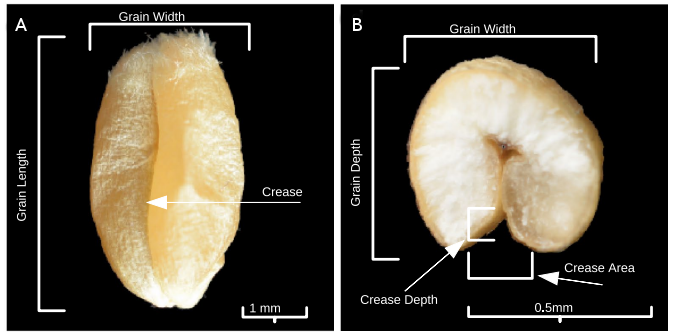
\includegraphics[width=17cm]{./images/seeds.png}
\caption{\label{fig:seeds}Wheat grain labelled (\emph{left}), wheat grain cut in half (\emph{right})}
\end{figure}

\section{Significance to Current Research}
\label{sec-1-3}
The biological interest in this area has been expressed in several areas of research \cite{Leigh2013}, it is proposed that the key to unlocking diversity in the wheat genus lies in these ancestor, undomesticated species \cite{Cockram2007}.

This research has the potential to be useful in several areas including: crop breeding; disease resistance; environmental stress.

The individual images in figure:\ref{fig:phylo} show, at a glance, the diversity and also the difference in the wild and cultivated (domesticated)
species. This work allows for these differences to be quantified and evaluated into useful metrics for answering research based questions.

\begin{figure}[htb]
\centering
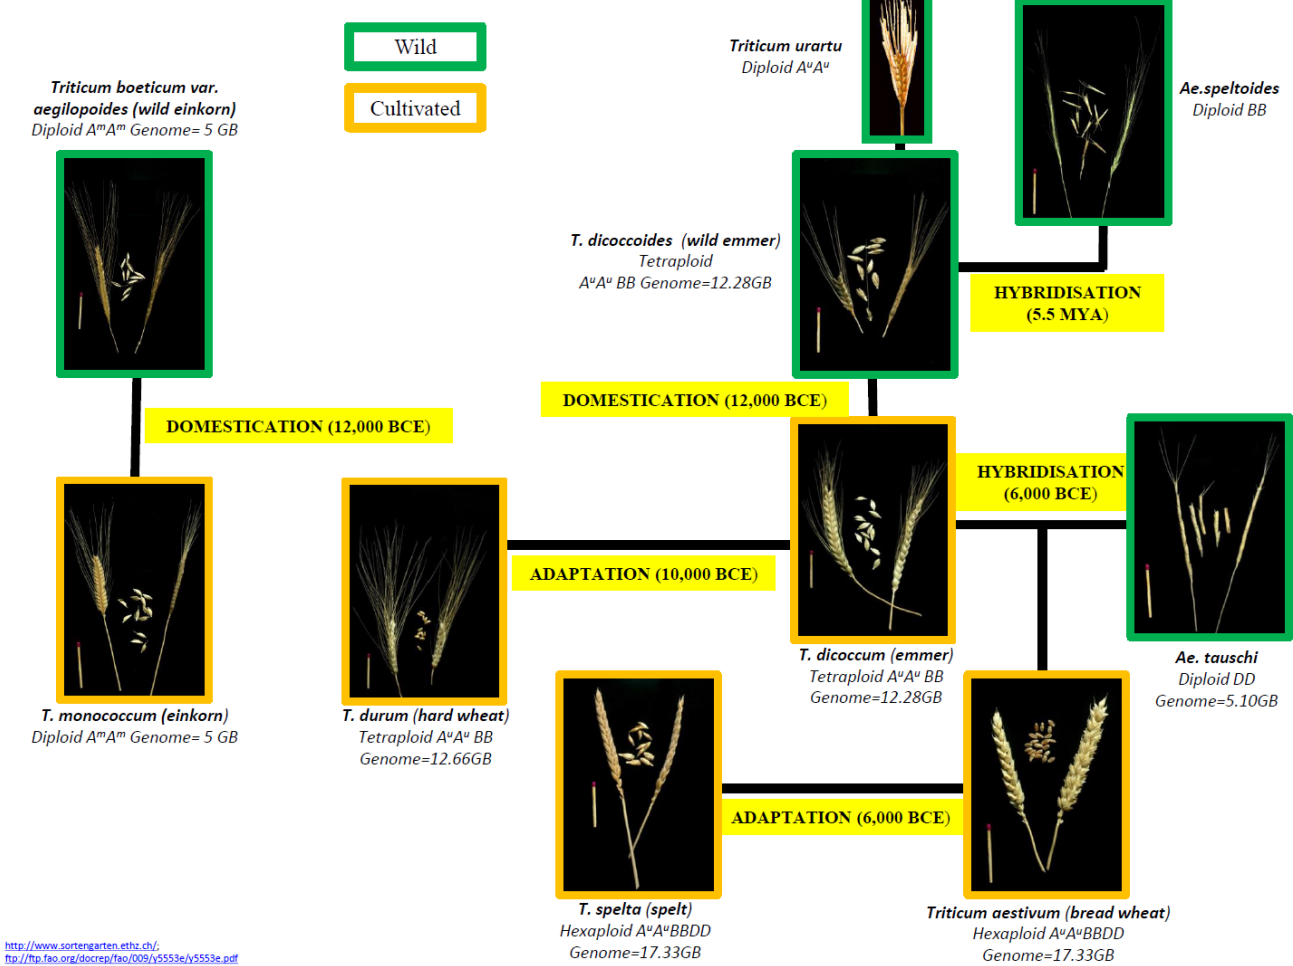
\includegraphics[width=17cm]{./images/philotree.png}
\caption{\label{fig:phylo}Phylogeny of wheat genotypes (Provided by Dr. Hugo Oliveira)}
\end{figure}

\section{Aim and Objectives}
\label{sec-1-4}

The overarching aim of this project has been to create several pieces of software which aid in answering the biologically significant questions outlined. As well as to prove/disprove the hypothesis stated below.

The software created is robust in order to duplicate results and is flexible as to allow for further studies to be carried out and to use the same method.

Novel additions have been made to existing image analysis libraries in order to make them more flexible for this project. Figure:\ref{fig:spikes} illustrates the range of diversity

\begin{figure}[htb]
\centering
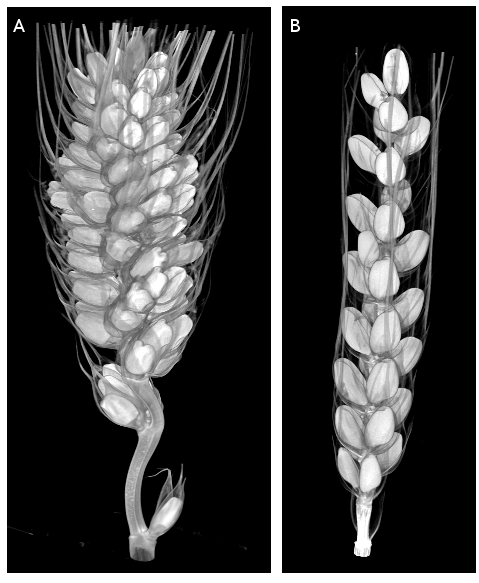
\includegraphics[width=11cm]{./images/spikes.png}
\caption{\label{fig:spikes}Two \textmu{}-CT scans of wheat spikes, showing diversity in Population, Compactum (6N) left, Durum right (4N)}
\end{figure}


Furthermore, the library written allows for easy data organisation and automation of otherwise difficult tasks such as concatenating data from multiple sources and graphing of information. Full documentation and integrated testing allows for a suite of tools which can be built upon in future and reduce the amount of effort required for similar studies to be carried out and analysed.

These aims have a focus on the phenotypic attributes generated from customised image analysis software \cite{Hughes2017} and can be seen in figure:\ref{fig:seeds}.

\section{Hypothesis}
\label{sec-1-5}
To provide a full spectrum of analysis the null-hypothesis of this work is presented as investigating if there are morphometric differences in the seeds of several wheat varieties outlined in figure:\ref{fig:phylo}.

The comparison pairs are as follows:

\begin{enumerate}
\item Monococcum Wild and Monococcum Domesticate
\item Dicoccoides and Dicoccum
\item Spelta and Aestivum
\item Dicoccum and Durum
\item Monococcum Wild and Dicoccoides
\end{enumerate}

\section{Problems Overview}
\label{sec-1-6}

The problems which this project tackles come in two flavours: Computational and Biological. As such keen awareness of these is needed to appreciate the novelty of this work.

\subsection{Biological Problems}
\label{sec-1-6-1}
Previous studies have been able to demonstrate that variation in wheat grain morphology can be partially explained, in 2010 Gegas et al. demonstrated this through a 99.4\% 2 component PCA \cite{Gegas2010}. However there is much left to do in terms of formal classifications and descriptions of these differences. This project deals with this problem through computational analysis.

Two effects run parallel in this study which requires acute biological knowledge of in order to make correct decisions:

\begin{enumerate}
\item The effects of ploidy in wheat.
\item The effects of domestication in wheat.
\end{enumerate}

Hypothesis are required to take into account, both of these effects so as not to misidentify results.

\subsection{Computational Problems}
\label{sec-1-6-2}
Using \textmu{}-CT data in plant sciences is becoming more and more common \cite{Tracy2017,Jhala2015,Hughes2017,Metzner2015} and whilst a lot of studies focus on the traits of grains specifically no formal model has been created, no accepted data format. This is a data engineering problem and the methods described in this project address this.

Further to data organisation, proposals are made for the statistical analysis which should be used. This allows for studies to become more robust and repeatable, thus strengthening the studies overall.

The biological material used in this research is much more diverse a population than has been previously studied with \textmu{}-CT image analysis, this requires current computer vision methods to be adapted in order to be accurate.

\section{Deliverables}
\label{sec-1-7}

This project provides three final deliveribles:

\begin{enumerate}
\item A flexible software suite written in \emph{Python} that provides a standardised method for analysing and interpreting \textmu{}-CT data output.
\item A Graphical User Interface (GUI) which offers a point and click method for data gathering, graphing and manipulating \textmu{}-CT data, using the library from deliverable 1 as a backend.
\item Answers to the proposed questions (hypothesis), the \emph{Results} and \emph{Discussion} sections of this report provides this.
\end{enumerate}

\chapter{Software Design, Implementation and Testing}
\label{sec-2}
This project made use of formal design methods and strict organisation whilst being flexible to change.
Overall the design took a hybridised form in order to best suit the scientific environment which this
domain specific software is built for.

\section{Software Development Methodology}
\label{sec-2-1}
Data analysis drove the direction of the project, as a result an agile methodology was adopted.
Weekly sprints were implemented as a list of "todo's", these were written on a Monday morning based off of the
previous week's list.

Critical self-evaluation was performed by means of a "one-man SCRUM" meeting, this is a technique which requires self-discipline in order to accurately find faults and areas for improvement.

\section{Functional Requirements}
\label{sec-2-2}
\subsection{Requirements for CT Analysing Library}
\label{sec-2-2-1}
\subsection{Requirements for CT GUI Application}
\label{sec-2-2-2}
\begin{itemize}
\item Useable by \emph{anyone}
\end{itemize}
\section{Version control}
\label{sec-2-3}
\section{Designing Process}
\label{sec-2-4}
\section{Documentation}
\label{sec-2-5}
The provided CT Analysing Library comes with "human-readable" format. Where most documentation generators (Doxygen, Pydocs, Javadocs etc.) implement very well structured and comprehensive documentation, the output is generally not very friendly and easy to read. Particularly for non-career-programmers. A core feature of these provided software implementations are that they are well suited for a biologist, researcher or statistician to use.

This documentation generator was purpose created, implemented in LISP and provided in listing:\ref{lst:docgen}.

Beyond this, inline commenting is provided for supplied software. Keeping in line with the agile development ethos the software is self-documented and self-evident. A brief example of this is shown in listing:\ref{lst:docexample}

Similarly, the documentation for using the CT GUI Application is based on feedback provided via user testing and Google form feedback data.
\section{Language Choice}
\label{sec-2-6}
\section{Software Library Choices}
\label{sec-2-7}
\section{Implementation}
\label{sec-2-8}

\section{Testing}
\label{sec-2-9}
\subsection{Feedback Forms}
\label{sec-2-9-1}
Feedback and constructive suggestions were made by researchers at the National Plant Phenomics Centre, these were submitted via the Google forms service\ldots{}
\subsection{Unit Testing CT Analysing Library}
\label{sec-2-9-2}

\begin{table}[htb]
\caption{\label{tab:unittest}Output of \emph{pytest} Unit Tests and results for CT Analysing Library}
\centering
\begin{tabularx}{\textwidth}{|l|X|r|}
\hline
\textbf{Result} & \textbf{Test} & \textbf{Duration}\\
\hline
\color{ForestGreen}Passed & CTData.py::test\_aggregate\_spike\_averages & 0.03\\
\hline
\color{ForestGreen}Passed & CTData.py::test\_clean\_data\_maximum\_removed & 0.00\\
\hline
\color{ForestGreen}Passed & CTData.py::test\_clean\_data\_minimum\_removed & 0.00\\
\hline
\color{ForestGreen}Passed & CTData.py::test\_load\_additional\_data & 1.30\\
\hline
\color{ForestGreen}Passed & CTData.py::test\_load\_additional\_data\_no\_data & 0.00\\
\hline
\color{ForestGreen}Passed & CTData.py::test\_load\_data & 0.13\\
\hline
\color{ForestGreen}Passed & CTData.py::test\_NoDataFoundException & 0.00\\
\hline
\color{ForestGreen}Passed & Data\_transforms.py::test\_box\_cox\_data & 0.01\\
\hline
\color{ForestGreen}Passed & Data\_transforms.py::test\_pca\_to\_table & 0.01\\
\hline
\color{ForestGreen}Passed & Data\_transforms.py::test\_perform\_pca & 0.02\\
\hline
\color{ForestGreen}Passed & Data\_transforms.py::test\_standardise\_data & 0.01\\
\hline
\color{ForestGreen}Passed & Graphing.py::test\_plot\_boxplot\_as\_dataframe & 0.05\\
\hline
\color{ForestGreen}Passed & Graphing.py::test\_plot\_boxplot\_as\_object & 0.05\\
\hline
\color{ForestGreen}Passed & Graphing.py::test\_plot\_difference\_of\_means & 0.11\\
\hline
\color{ForestGreen}Passed & Graphing.py::test\_plot\_histogram\_as\_dataframe & 0.02\\
\hline
\color{ForestGreen}Passed & Graphing.py::test\_plot\_histogram\_as\_object & 0.02\\
\hline
\color{ForestGreen}Passed & Graphing.py::test\_plot\_pca & 0.17\\
\hline
\color{ForestGreen}Passed & Graphing.py::test\_plot\_qqplot & 0.00\\
\hline
\color{ForestGreen}Passed & Statistical\_tests.py::test\_baysian\_hypothesis\_test & 10.76\\
\hline
\color{ForestGreen}Passed & Statistical\_tests.py::test\_t\_test & 0.00\\
\hline
\color{ForestGreen}Passed & Statistical\_tests.py::test\_test\_normality & 0.00\\
\hline
\end{tabularx}
\end{table}

\subsection{Unit Testing CT GUI Application}
\label{sec-2-9-3}
\chapter{Methods and Solutions}
\label{sec-3}
\section{Data Pipeline}
\label{sec-3-1}

\begin{center}
\begin{figure}[htb]
\centering
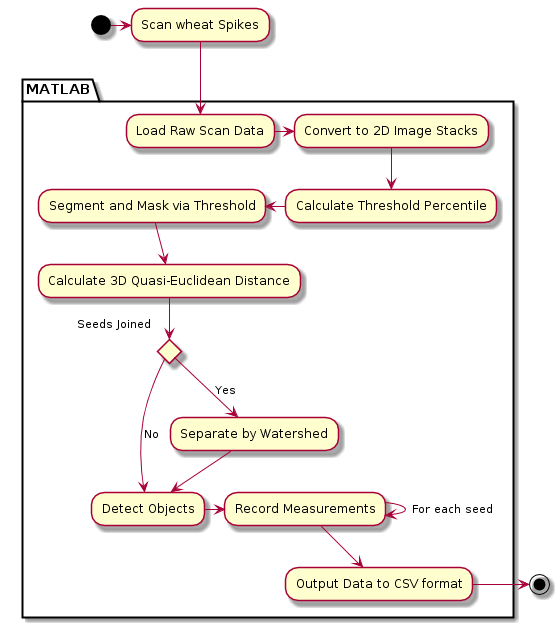
\includegraphics[width=10cm]{./images/matlab.png}
\caption{\label{fig:matlab}Image Processing Pipeline}
\end{figure}
\end{center}

\section{Image Analysis Methods}
\label{sec-3-2}
\subsection{New Watershed Algorithm}
\label{sec-3-2-1}

In order to solve the problem of misidentified and joint seeds, from the primitive collection,
a  \emph{quasi-euclidean} distance transform was implemented into the analysis pipeline (figure:\ref{fig:matlab}). This provided much better results than the previous
\emph{chessboard} transform which had been successful on more uniform data in previous studies \cite{Hughes2017}.

\subsubsection{Quasi-Euclidean algorithm}
\label{sec-3-2-1-1}

This algorithm measures the total euclidean distance along a set of horizontal, vertical and diagonal
line segments \cite{Pfaltz1966}.

\begin{equation}
\label{eqn:qe}
\left | x_1 - x_2 \right | + (\sqrt{2}-1), \left | x_1 - x_2 \right | >\left | y_1 - y_2 \right | (\sqrt{2}-1) \left | x_1 - x_2 \right | ,\textup{otherwise}
\end{equation}


In order to apply this to a 3D space Kleinberg's method is used  \cite{Kleinberg1997}. This allows for nearest neighbour pixels to be sorted by $k$-dimensional trees
and enabling fast distance transforms via Rosenfeld and Pfaltz's \emph{quasi-euclidean} method stated in equation:\ref{eqn:qe}.
\subsubsection{Effect of Enhanced Watershed algorithm}
\label{sec-3-2-1-2}
\begin{center}
\begin{figure}[htb]
\centering
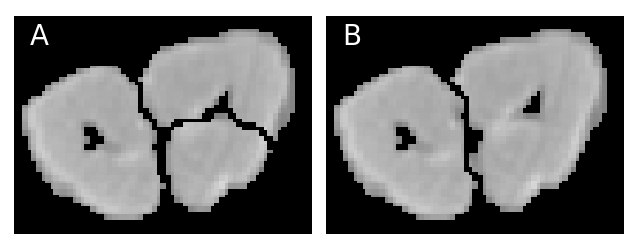
\includegraphics[width=10cm]{./images/chess_quasi.png}
\caption{\label{fig:qe}\emph{A} showing the chessboard method, \emph{B} improved quasi-euclidean method}
\end{figure}
\end{center}

\section{CT Analysing Library Methods}
\label{sec-3-3}
\section{CT GUI Application Methods}
\label{sec-3-4}
\section{Data Analysis Methods}
\label{sec-3-5}
\begin{center}
\begin{figure}[htb]
\centering
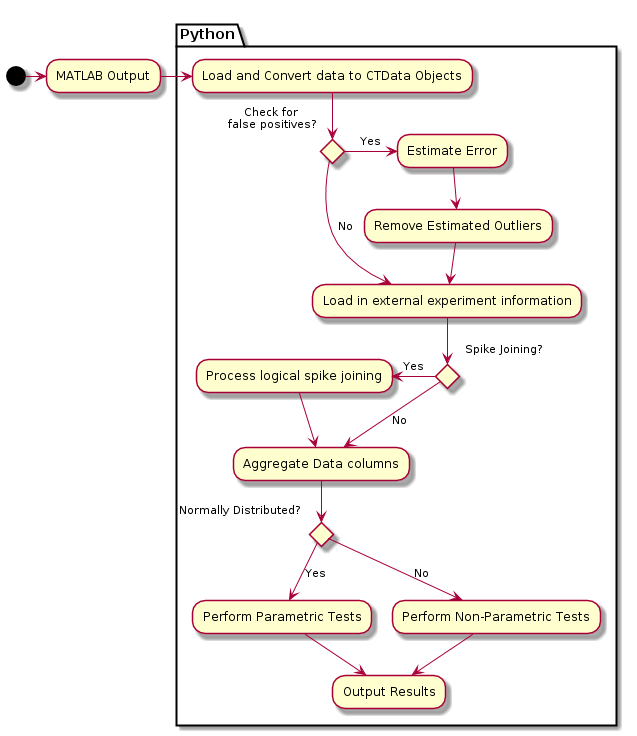
\includegraphics[width=10cm]{./images/pipeline.png}
\caption{\label{fig:pipeline}How data is integrated with the CT Analysing Library}
\end{figure}
\end{center}

\chapter{Results}
\label{sec-4}
\chapter{Discussion}
\label{sec-5}
\section{Similar Research}
\label{sec-5-1}
\section{Alternate Solutions}
\label{sec-5-2}

\chapter{Critical Evaluation}
\label{sec-6}
\section{Organisational Methods}
\label{sec-6-1}
\section{Relevance to Degree}
\label{sec-6-2}
\section{Time Management}
\label{sec-6-3}
\section{Collaborative Work}
\label{sec-6-4}
\section{Other Issues}
\label{sec-6-5}

\chapter{Appendix}
\label{sec-7}
\section{\emph{Software Packages Used}}
\label{sec-7-1}

\subsection{Libraries}
\label{sec-7-1-1}
\begin{table}[htb]
\caption{\label{tab:software}Software libraries used}
\centering
\begin{tabularx}{\textwidth}{|X|X|X|}
\hline
MATLAB Image Processing Toolbox & Numpy & Matplotlib\\
\hline
Seaborn & Scipy & Sklearn\\
\hline
Statsmodels & Pymc3 & Xlrd\\
\hline
PyQt5 &  & \\
\hline
\end{tabularx}
\end{table}

\subsection{Tools}
\label{sec-7-1-2}
\begin{table}[htb]
\caption{\label{tab:softwareused}Software tools used}
\centering
\begin{tabularx}{\textwidth}{|X|X|X|}
\hline
MATLAB & Python Debugger (PDB) & IPython\\
\hline
Emacs & git & org-mode\\
\hline
Tomviz & ImageJ & \\
\hline
\end{tabularx}
\end{table}

\section{\emph{Glossary}}
\label{sec-7-2}
\begin{table}[htb]
\caption{\label{tab:glossary}Dictionary for Terms and acronyms}
\centering
\begin{tabularx}{\textwidth}{|l|X|}
\hline
\textbf{Term} & \textbf{Definition}\\
\hline
\textmu{}-CT & Micro Computed Tomography\\
\hline
Genotype & A genetically distinct individual or group\\
\hline
Phenotype & A physical/measurable trait\\
\hline
Alleles & A variant of a gene\\
\hline
Genus & Classification ranking, below the \emph{family} grouping\\
\hline
Genome & The complete genetic make up of an organism, which defines its individuality\\
\hline
Morphometric & The shape and form of an organism\\
\hline
GUI & Graphical User Interface\\
\hline
PCA & Principal Component Analysis\\
\hline
\end{tabularx}
\end{table}


\section{\emph{Code Segments and Examples}}
\label{sec-7-3}
\subsection{MATLAB Watershedding}
\label{sec-7-3-1}

\begin{listing}[H]
\begin{minted}[]{octave}
function [W] = watershedSplit3D(A)
  % Takes image stack A and splits it into stack W
  % Convert to BW
  bw = logical(A);
  % Create variable for opening and closing
  se = strel('disk', 5);
  % Minimise object missshapen-ness
  bw = imerode(bw, se);
  bw = imdilate(bw, se);
  % Fill in any left over holes
  bw = imfill(bw,4,'holes');
  % Use chessboard for distance calculation for more refined splitting
  chessboard = -bwdist(~bw, 'quasi-euclidean');
  % Modify the intensity of our bwdist to produce chessboard2
  mask = imextendedmin(chessboard, 2);
  chessboard2 = imimposemin(chessboard, mask);
  % Calculate watershed based on the modified chessboard
  Ld2 = watershed(chessboard2);
  % Take original image and add on the lines calculated for splitting
  W = A;
  W(Ld2 == 0) = 0;
end
\end{minted}
\caption{\label{lst:ws}MATLAB Watershedding function}
\end{listing}

\subsection{Custom Documentation Generator}
\label{sec-7-3-2}
\begin{listing}[H]
\begin{minted}[]{common-lisp}
(defun populate-org-buffer (buffer filename root)
  (goto-char (point-min))
  (let ((to-insert (concat "* " (replace-regexp-in-string root "" filename) "\n") ))
    (while (re-search-forward
            (rx (group (or "def" "class"))
                space
                (group (+ (not (any "()"))))
                (? "(" (* nonl) "):" (+ "\n") (+ space)
                   (= 3 "\"")
                   (group (+? anything))
                   (= 3 "\"")))
            nil 'noerror)
      (setq to-insert
            (concat
             to-insert
             (if (string= "class" (match-string 1))
                 "** "
               "*** ")
             (match-string 2)
             "\n"
             (and (match-string 3)
                  (concat (match-string 3) "\n")))))
    (with-current-buffer buffer
      (insert to-insert))))

(defun org-documentation-from-dir (&optional dir)
  (interactive)
  (let* ((dir  (or dir (read-directory-name "Choose base directory: ")))
         (files (directory-files-recursively dir "\py$"))
         (doc-buf (get-buffer-create "org-docs")))
    (dolist (file files)
      (with-temp-buffer
        (insert-file-contents file)
        (populate-org-buffer doc-buf file dir)))
    (with-current-buffer doc-buf
      (org-mode))))
\end{minted}
\caption{\label{lst:docgen}Custom lisp code for generating easy to read documentation}
\end{listing}

\clearpage
\subsection{Self-Documenting Code Example}
\label{sec-7-3-3}
\begin{listing}[H]
\begin{minted}[]{python}
def get_spike_info(self, excel_file, join_column='Folder#'):
    """
    This function should do something akin to adding additional
    information to the data frame

    @note there is some confusion in the NPPC about whether to use
    folder name or file name as the unique id when this is made into
    end-user software, a toggle should be added to allow this

    @param excel_file a file to attach and read data from
    @param join_column if the column for joining data is
    different then it should be stated
    """
    try:
        # Grab the linking excel file
        info = pd.read_excel(excel_file,
                             index_col='Folder#')

        features = list(info.columns)
        # Lambda to look up the feature in excel spreadsheet
        def look_up(x, y): return info.loc[x['folderid']][y]

        # Lambda form a series (data row) and apply it to dataframe
        def gather_data(x): return pd.Series(
            [look_up(x, y) for y in features])

        self.df[features] = self.df.apply(gather_data, axis=1)
    except KeyError as e:
        print('Error matching data')
        print(e)
        raise NoDataFoundException
    except AttributeError as e:
        print(e)
        raise NoDataFoundException
\end{minted}
\caption{\label{lst:docexample}Example of code documentation and readability from \emph{data\_transforms.py}}
\end{listing}

\clearpage
\bibliography{library}
\bibliographystyle{IEEEannotU}
% Emacs 25.3.50.2 (Org mode 8.2.10)
\end{document}
